\section{Results \& Discussion}
only triangle plots

\subsection{Signatures of \acp{IMBH} in action space}\label{results}
After investigating the orbits at given actions and the time evolution of the integrals of motion we consider all actions and other integrals of motion at our given snapshots. We have a look at the energies and angular momenta of the stars and compare them with the radial actions. Our main goal is to find any systematic signatures for the simulations with \acp{IMBH} that can be considered as the direct evidence of the dynamical effect of the \ac{IMBH} itself. For this reason we investigate selected stars which show an abnormal behaviour in above-mentioned plots and compare them to the rest of the data to see where we find them.

\begin{figure}[htbp]
\centering
	\begin{subfigure}{0.475\textwidth}
		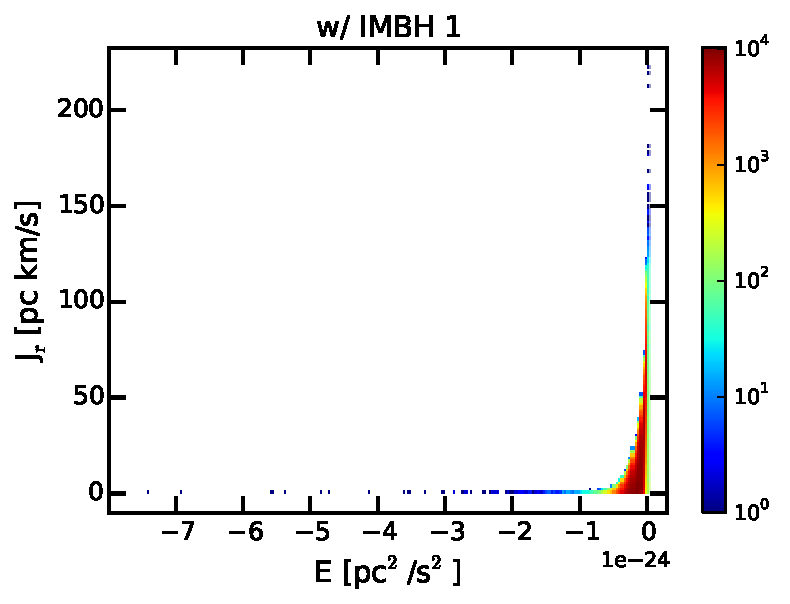
\includegraphics[width=\textwidth]{Plots/E_J_r_hist_IMBH1.pdf}
		\caption{SIM 1}
		\label{fig:E_J_r_hist_IMBH1}
	\end{subfigure}
	\hfill
	\begin{subfigure}{0.475\textwidth}
		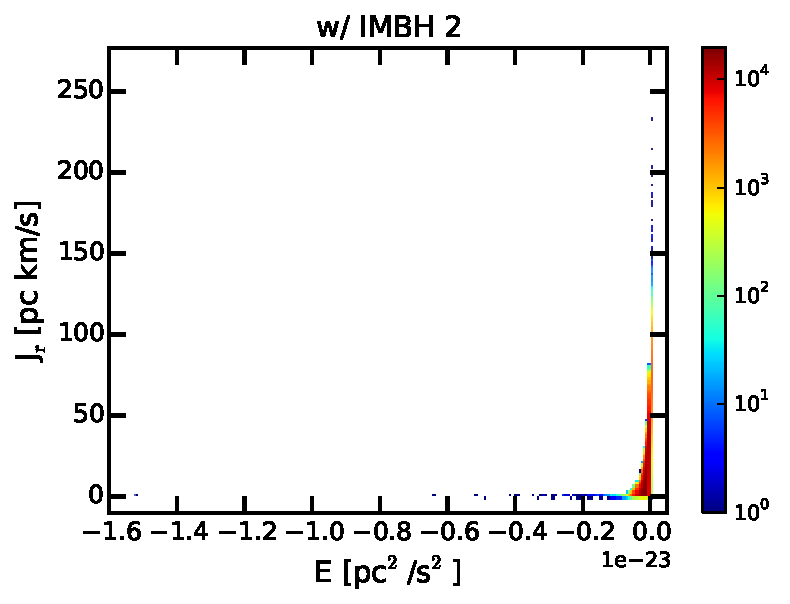
\includegraphics[width=\textwidth]{Plots/E_J_r_hist_IMBH2.pdf}
		\caption{SIM 2}
		\label{fig:E_J_r_hist_IMBH2}
	\end{subfigure}
	\vskip\baselineskip
	\begin{subfigure}{0.475\textwidth}
		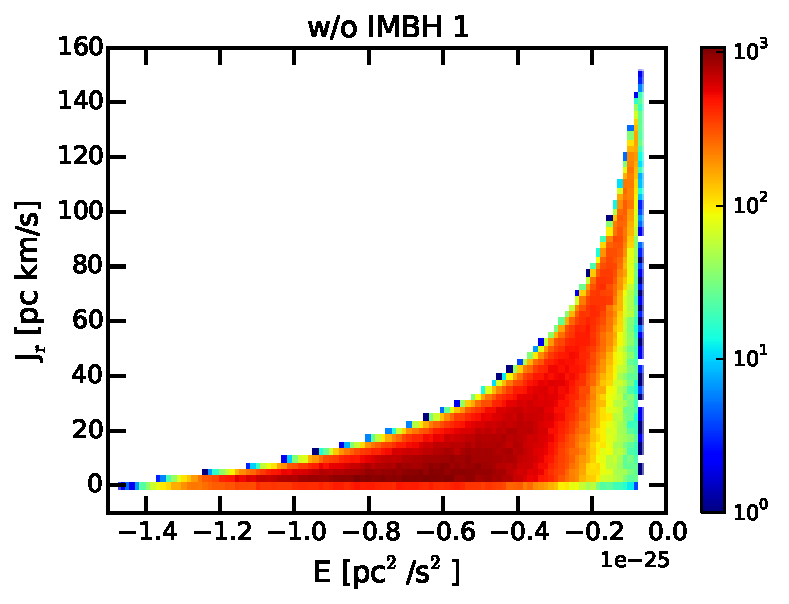
\includegraphics[width=\textwidth]{Plots/E_J_r_hist_noIMBH1.pdf}
		\caption{SIM 3}
		\label{fig:E_J_r_hist_noIMBH1}
	\end{subfigure}
	\hfill
	\begin{subfigure}{0.475\textwidth}
		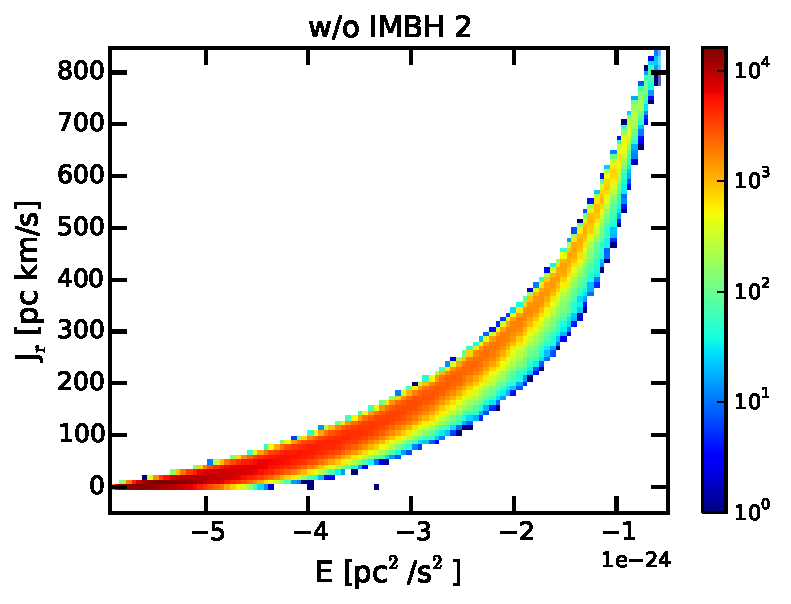
\includegraphics[width=\textwidth]{Plots/E_J_r_hist_noIMBH2.pdf}
		\caption{SIM 4}
		\label{fig:E_J_r_hist_noIMBH2}
	\end{subfigure}
	\caption{Radial action over energy. In \ref{fig:E_J_r_hist_IMBH1} and \ref{fig:E_J_r_hist_IMBH2} it is plotted for both simulations with \ac{IMBH} and the lower ones are for the simulation without \ac{IMBH}. We find the crescent shape from \ref{fig:E_J_r_hist_noIMBH1} and \ref{fig:E_J_r_hist_noIMBH2} clearly in \ref{fig:E_J_r_hist_IMBH1} and \ref{fig:E_J_r_hist_IMBH2}. But in SIM 1 and SIM 2 there are some stars differing from this shape. Some have high energy with no radial actions (henceforth referred to as group 1) while others have high radial actions with nearly no energy (henceforth group 2).}
	\label{fig:E_J_r_hist}
\end{figure}	
In \ref{fig:E_J_r_hist} we plot the radial action over the energy of the star as histograms for all \acp{GC}. We see clearly some stars outside of the moon shape. They have either no radial action and high energy(below \(-4 \cdot10^{-24}\) \(pc^2/s^2\)) or nearly no energy and high radial action (above 500 pc km/s). 
\par The first group of stars of SIM 1 contains 38 of the nearest 110 stars including the innermost 15 stars. Since they have really low (nearly 0) radial actions they are on circular orbits. The nearest 15 on circular orbits around the \ac{IMBH} are certainly locked to the \ac{IMBH}. That is why we do not see this signature for SIM 3 and SIM 4. The other stars of this group are likely to be locked to the \ac{IMBH} as well while the rest of the near stars which are not in this group seem to be near to or in their pericentre on more elliptic orbits and therefore not locked to the \ac{IMBH}. 
\par The other group of stars with high radial actions and nearly no energy can not be clearly related to the \ac{IMBH}. They are the furthermost stars of the snapshot. All are in their apocentre on very elliptic orbits (\color{red} calculate ellipticity? \color{black}). This ellipticity could be caused by the \ac{IMBH} but since most of their pericentres are at a few pc we can not assume much interaction with the \ac{IMBH} for those stars. Another reason that these stars do not occur in this way in SIM 3 and SIM 4 can be due to different truncation prescriptions used in the simulations (see graph \ref{fig:anisotropy_param}). These stars are nearly outside of the \acp{GC} and have about zero energy so they could have been excluded in SIM 3 and SIM 4. 


\begin{figure}[htbp]
\centering
	\begin{subfigure}{0.475\textwidth}
		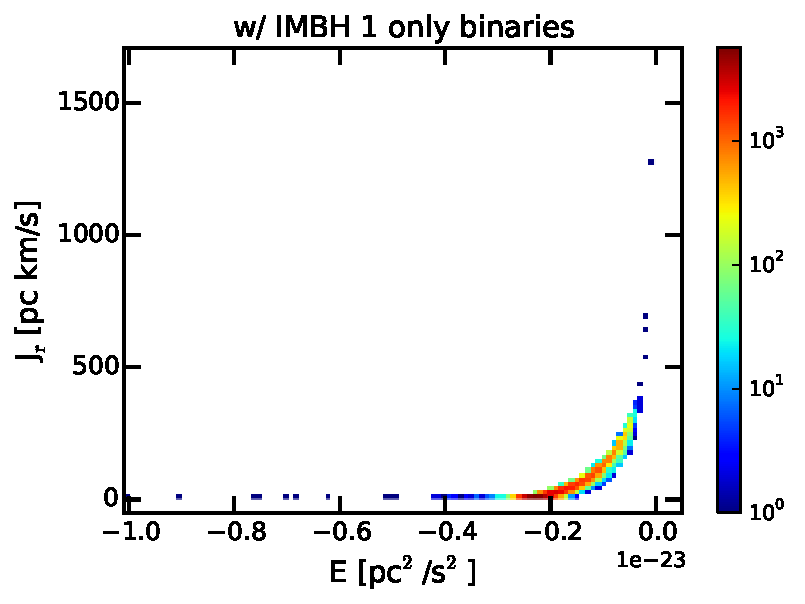
\includegraphics[width=\textwidth]{Plots/E_J_r_hist_bins_IMBH1.pdf}
		\caption{SIM 1}
		\label{fig:E_J_r_hist_bins_IMBH1}
	\end{subfigure}
	\hfill
	\begin{subfigure}{0.475\textwidth}
		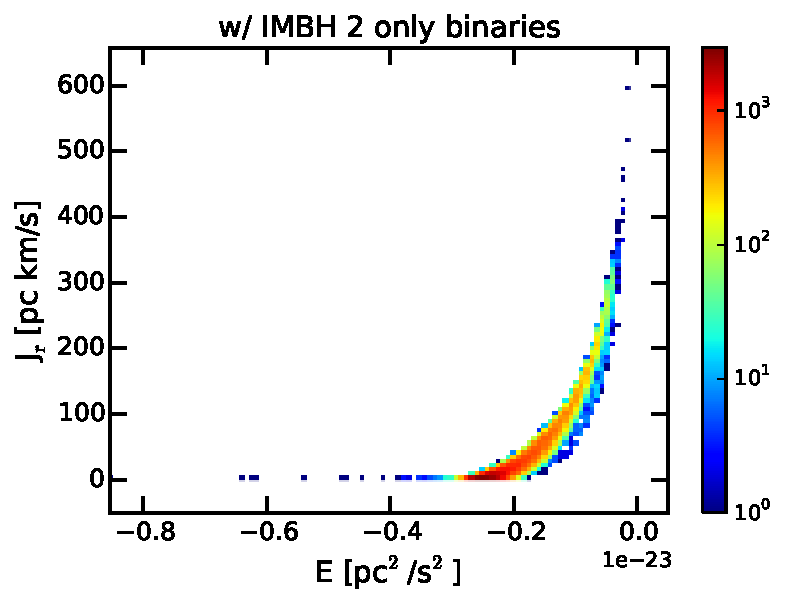
\includegraphics[width=\textwidth]{Plots/E_J_r_hist_bins_IMBH2.pdf}
		\caption{SIM 2}
		\label{fig:E_J_r_hist_bins_IMBH2}
	\end{subfigure}
	\vskip\baselineskip
	\begin{subfigure}{0.475\textwidth}
		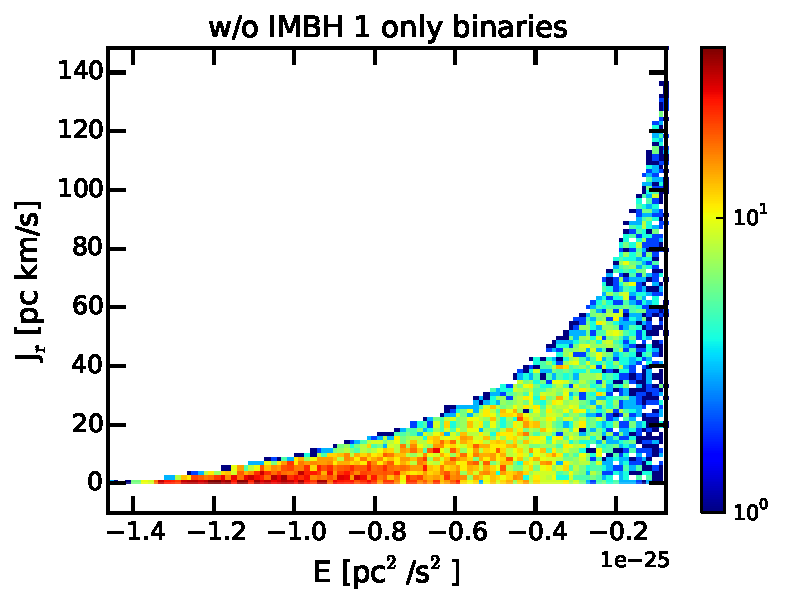
\includegraphics[width=\textwidth]{Plots/E_J_r_hist_bins_noIMBH1.pdf}
		\caption{SIM 3}
		\label{fig:E_J_r_hist_bins_noIMBH1}
	\end{subfigure}
	\hfill
	\begin{subfigure}{0.475\textwidth}
		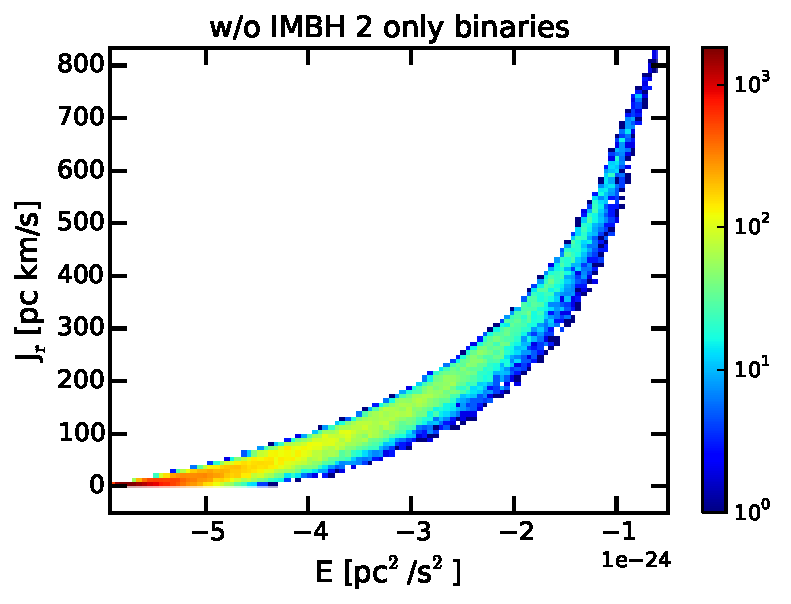
\includegraphics[width=\textwidth]{Plots/E_J_r_hist_bins_noIMBH2.pdf}
		\caption{SIM 4}
		\label{fig:E_J_r_hist_bins_noIMBH2}
	\end{subfigure}
	\caption{Radial action over energy only of binary systems. We see the same distribution of stars as in \ref{fig:E_J_r_hist}.}
	\label{fig:E_J_r_bins_hist}
\end{figure}

\par We might get these high energies from former binaries which were divided earlier. One of the stars could have been captured on a circular orbit near the centre while the other could have been left on an unbound orbit and have left the system. To check this we will plot the same values only for our actual binary systems. As we see in \ref{fig:E_J_r_bins_hist} the binary systems are behaving like single stars. There is no signature that the divergent stars are leftovers of former binaries. 


\begin{figure}[htbp]
\centering
	\begin{subfigure}{0.475\textwidth}
		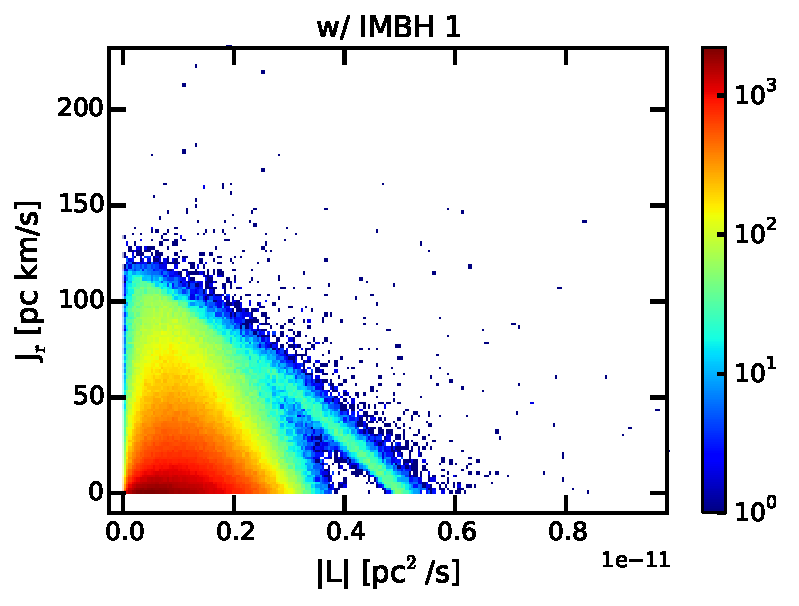
\includegraphics[width=\textwidth]{Plots/L_J_r_hist_IMBH1.pdf}
		\caption{SIM 1}
		\label{fig:L_J_r_hist_IMBH1}
	\end{subfigure}
	\hfill
	\begin{subfigure}{0.475\textwidth}
		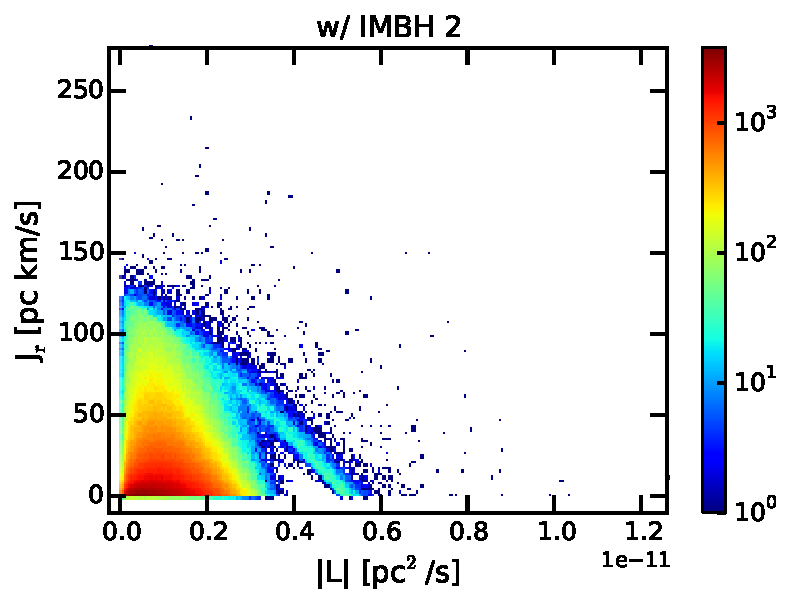
\includegraphics[width=\textwidth]{Plots/L_J_r_hist_IMBH2.pdf}
		\caption{SIM 2}
		\label{fig:L_J_r_hist_IMBH2}
	\end{subfigure}
	\vskip\baselineskip
	\begin{subfigure}{0.475\textwidth}
		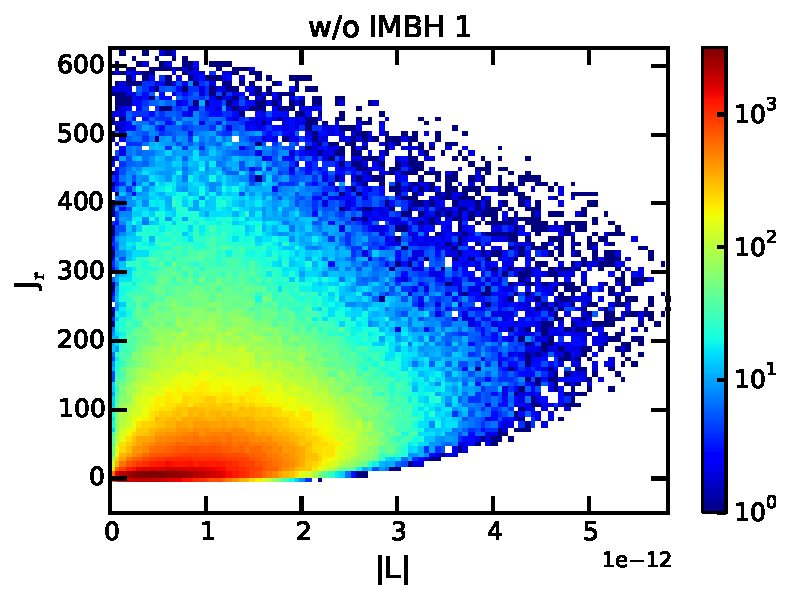
\includegraphics[width=\textwidth]{Plots/L_J_r_hist_noIMBH1.pdf}
		\caption{SIM 3}
		\label{fig:L_J_r_hist_noIMBH1}
	\end{subfigure}
	\hfill
	\begin{subfigure}{0.475\textwidth}
		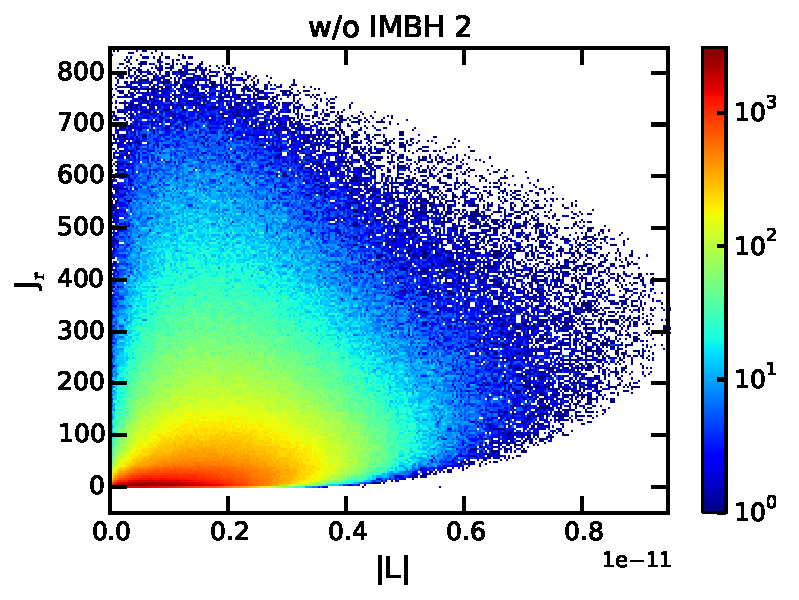
\includegraphics[width=\textwidth]{Plots/L_J_r_hist_noIMBH2.pdf}
		\caption{SIM 4}
		\label{fig:L_J_r_hist_noIMBH2}
	\end{subfigure}
	\caption{Radial action over angular momentum. \ref{fig:L_J_r_hist_noIMBH1} and \ref{fig:L_J_r_hist_noIMBH2} look again very similar to each other with no recognizable substructure. In \ref{fig:L_J_r_hist_IMBH1} and \ref{fig:L_J_r_hist_IMBH2} there are stars above the main shape. In the shape we can clearly see a substructure from about 0.3 to about 0.5 pc\(^2\)/s in nearly the whole radial action range. \color{red} DO YOU HAVE ANY IDEA WHAT STARS COULD BE THERE??? \color{black}}
	\label{fig:L_J_r_hist}
\end{figure}
\par Next we plot the radial actions over the absolute angular momenta of the stars of the simulations again as histograms. In \ref{fig:L_J_r_hist} we can see a triangular shape which seems characteristic. Inside this shape we see some substructure in the \acp{GC} with \ac{IMBH}. The stars outside the shape are the stars of group 2 which we see in \ref{fig:E_J_r_hist} and \ref{fig:E_J_r_bins_hist} as the stars with no energy and high radial actions. Obviously they don't seem to have a specific angular momentum. We do not know how to identify the stars in the substructure. There could be a mass-dependent correlation due to dynamical mass segregation.

\par We extract these divergent stars and determine their properties. First we check the positions of their actions depending on their guiding star radii.
\begin{figure}
\centering
	\begin{subfigure}{0.475\textwidth}
		\centering
		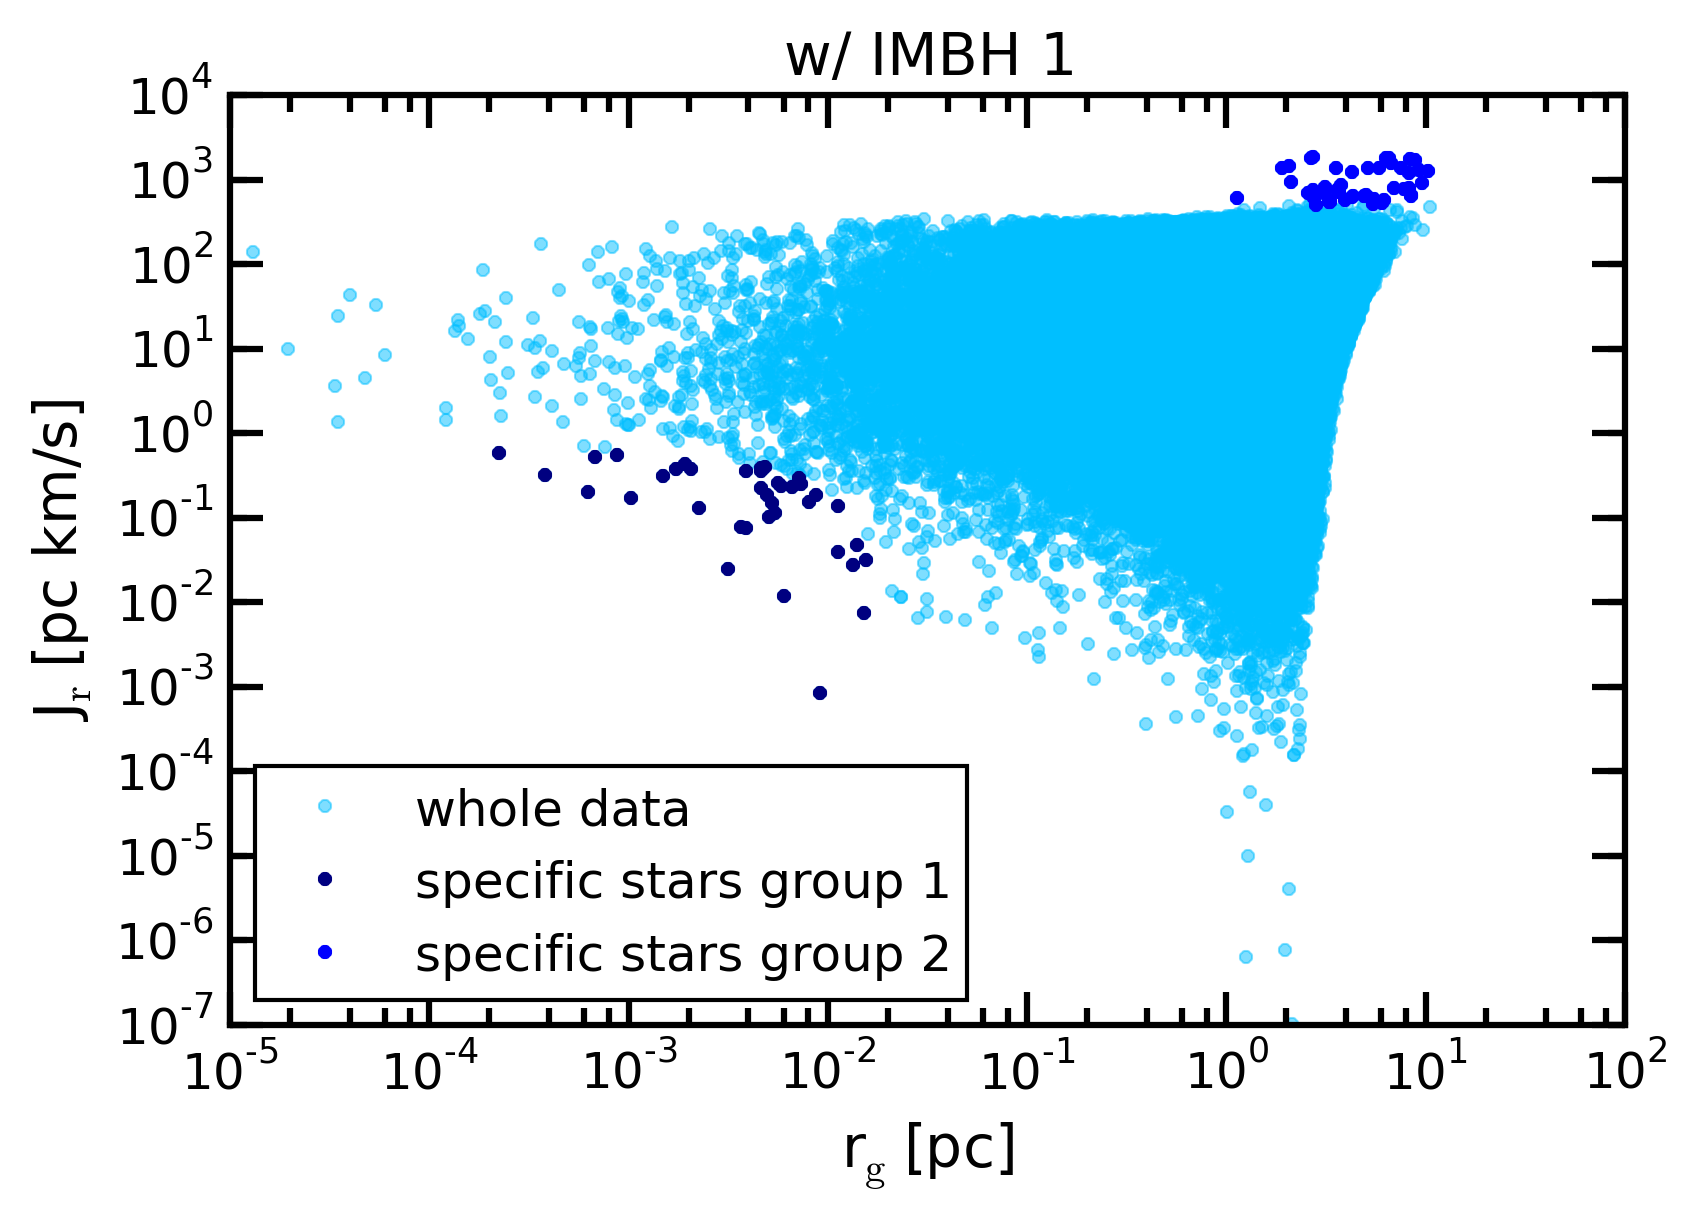
\includegraphics[width=\textwidth]{Plots/r_g_J_r_IMBH1.png}
		\caption{SIM 1}
		\label{fig:r_g_J_r_IMBH1}
	\end{subfigure}
	\hfill
	\begin{subfigure}{0.475\textwidth}
		\centering
		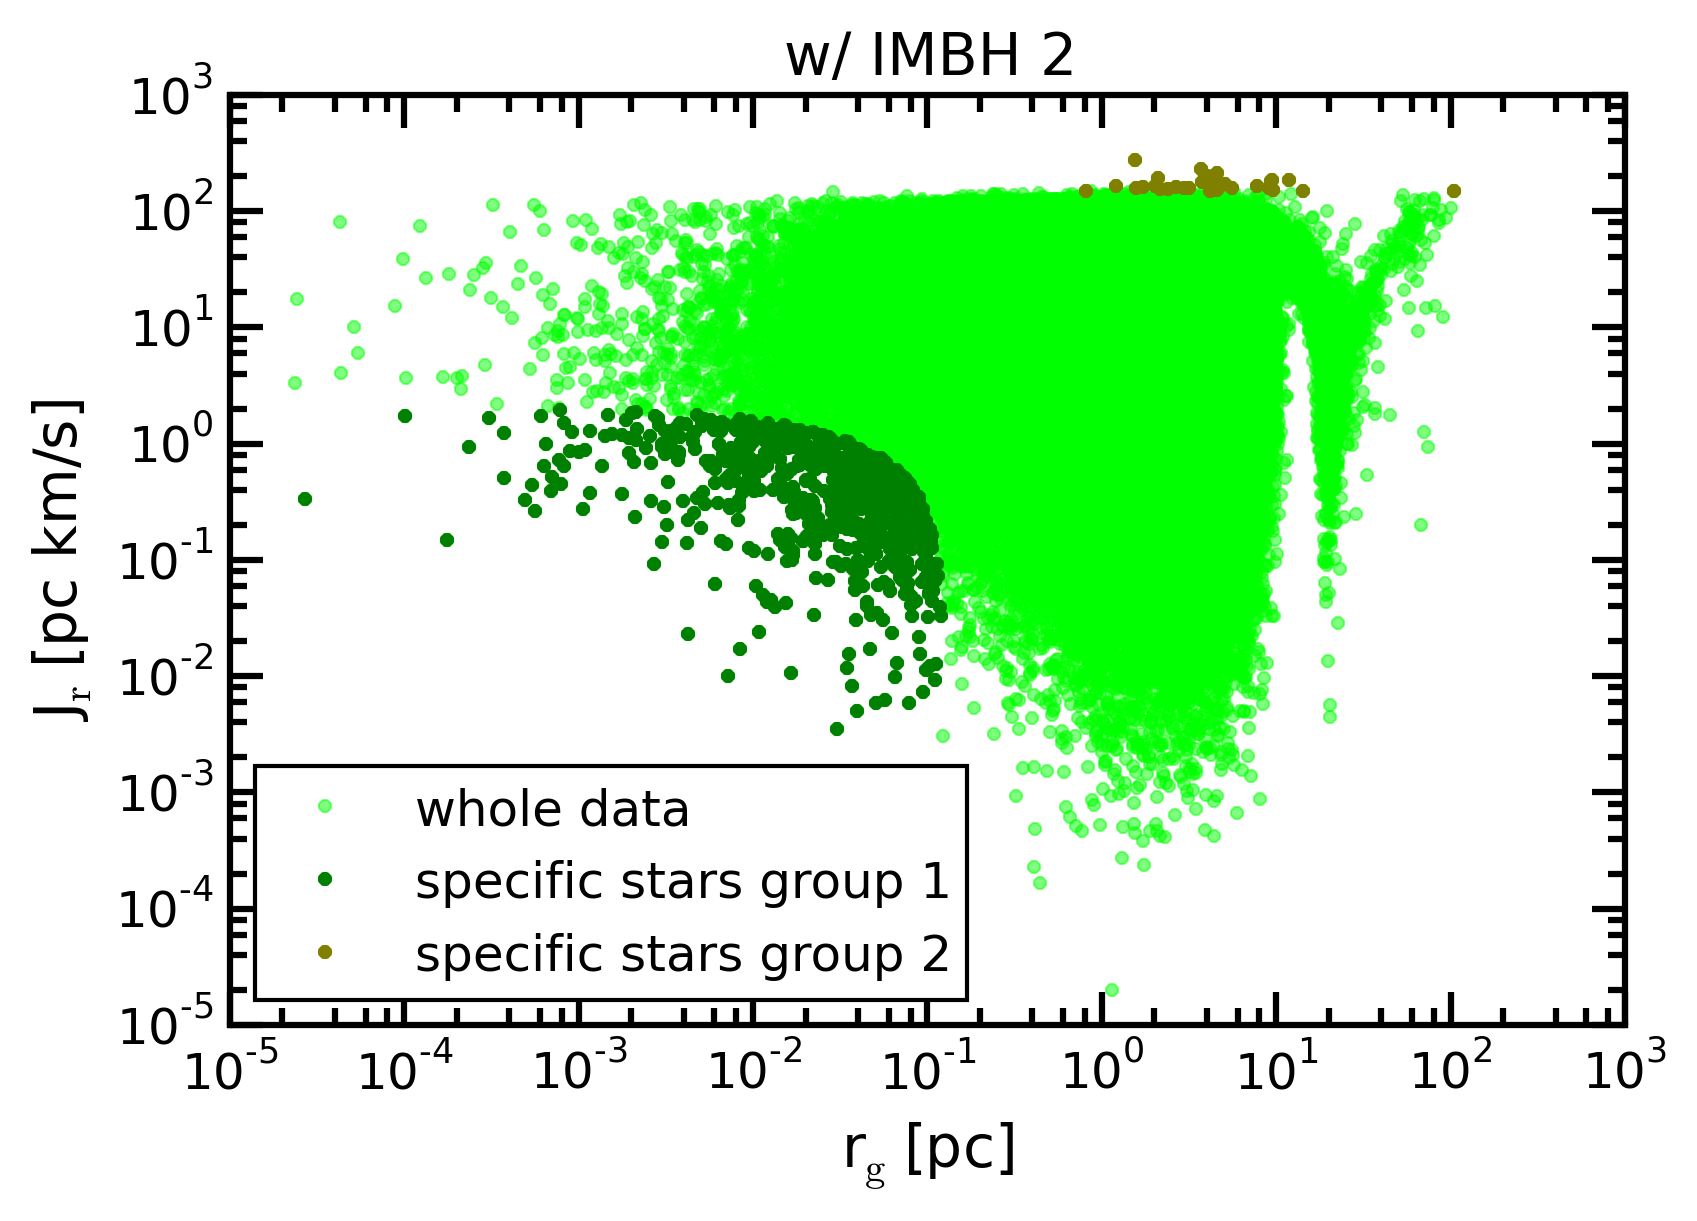
\includegraphics[width=\textwidth]{Plots/r_g_J_r_IMBH2.png}
		\caption{SIM 2}
		\label{fig:r_g_J_r_IMBH2}
	\end{subfigure}
	\vskip\baselineskip
	\begin{subfigure}{0.475\textwidth}
		\centering
		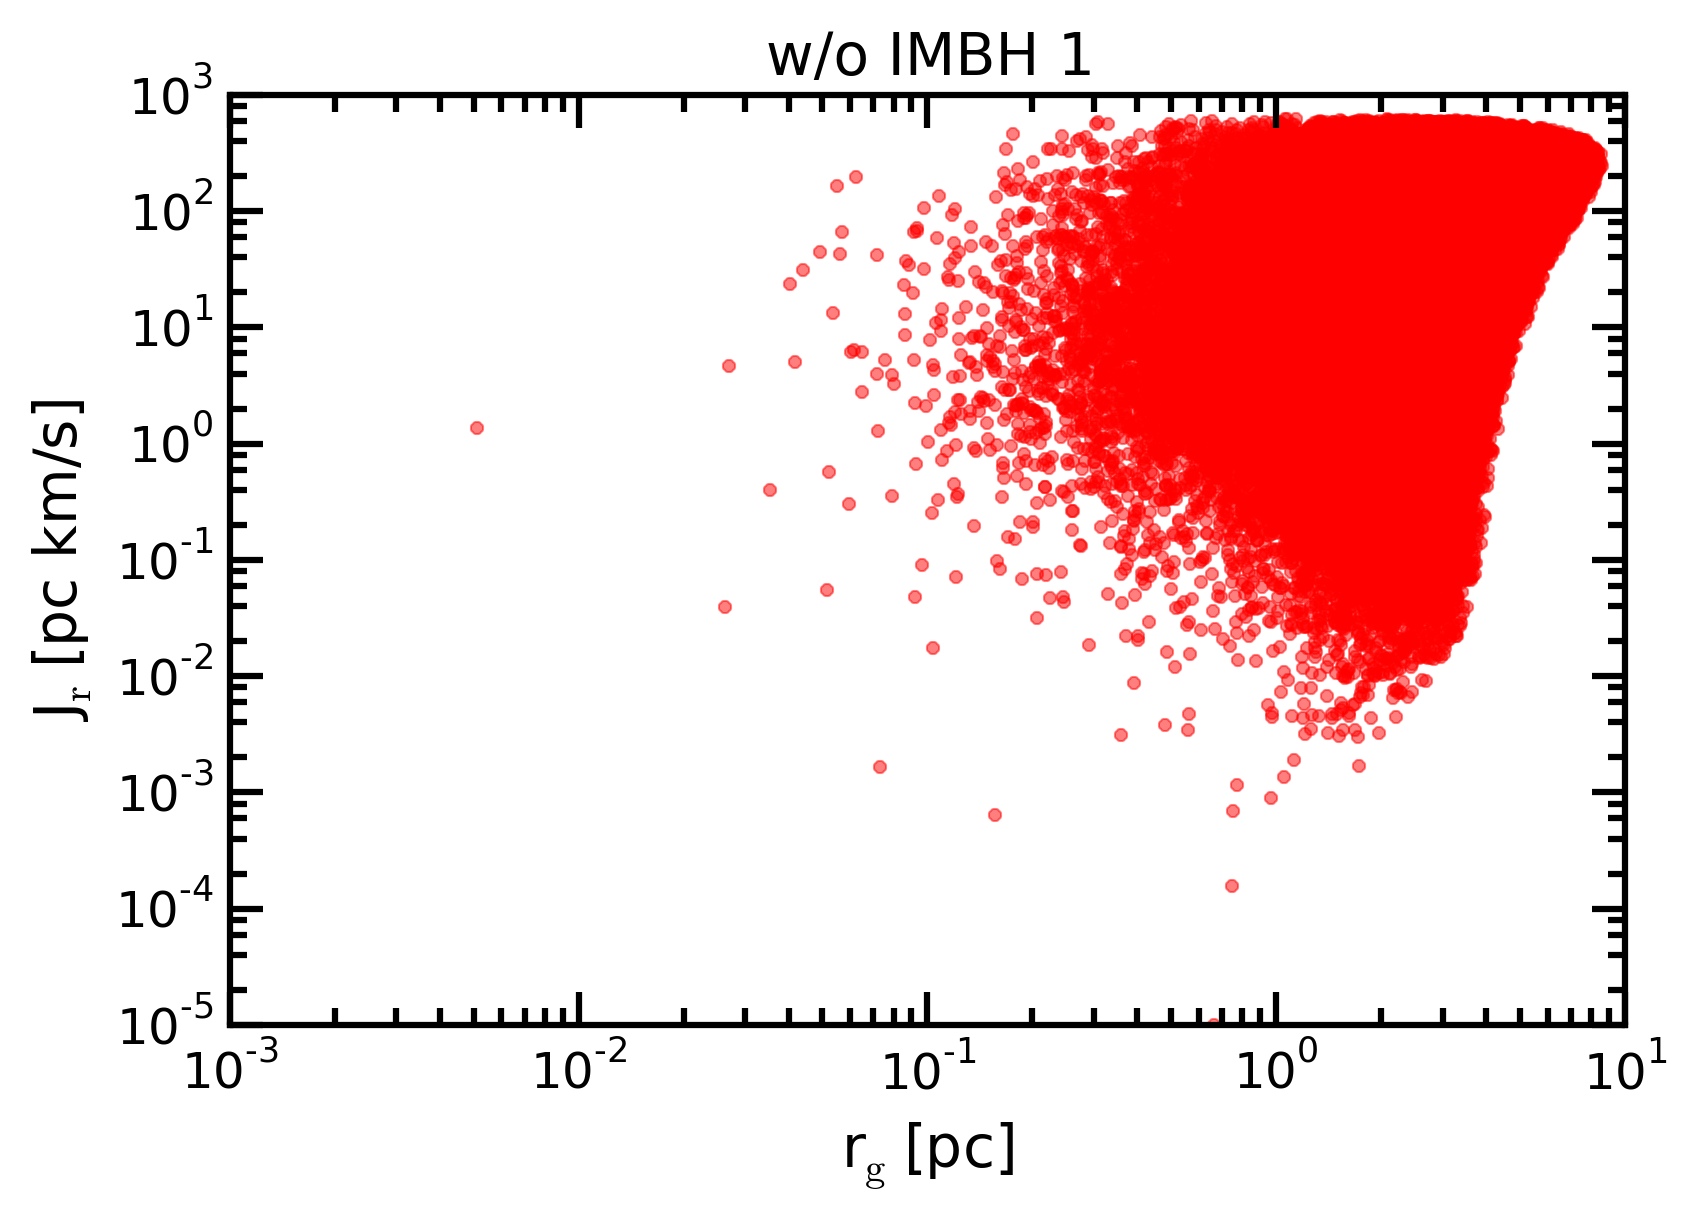
\includegraphics[width=\textwidth]{Plots/r_g_J_r_noIMBH1.png}
		\caption{SIM 3}
		\label{fig:r_g_J_r_noIMBH1}
	\end{subfigure}
	\hfill
	\begin{subfigure}{0.475\textwidth}
		\centering
		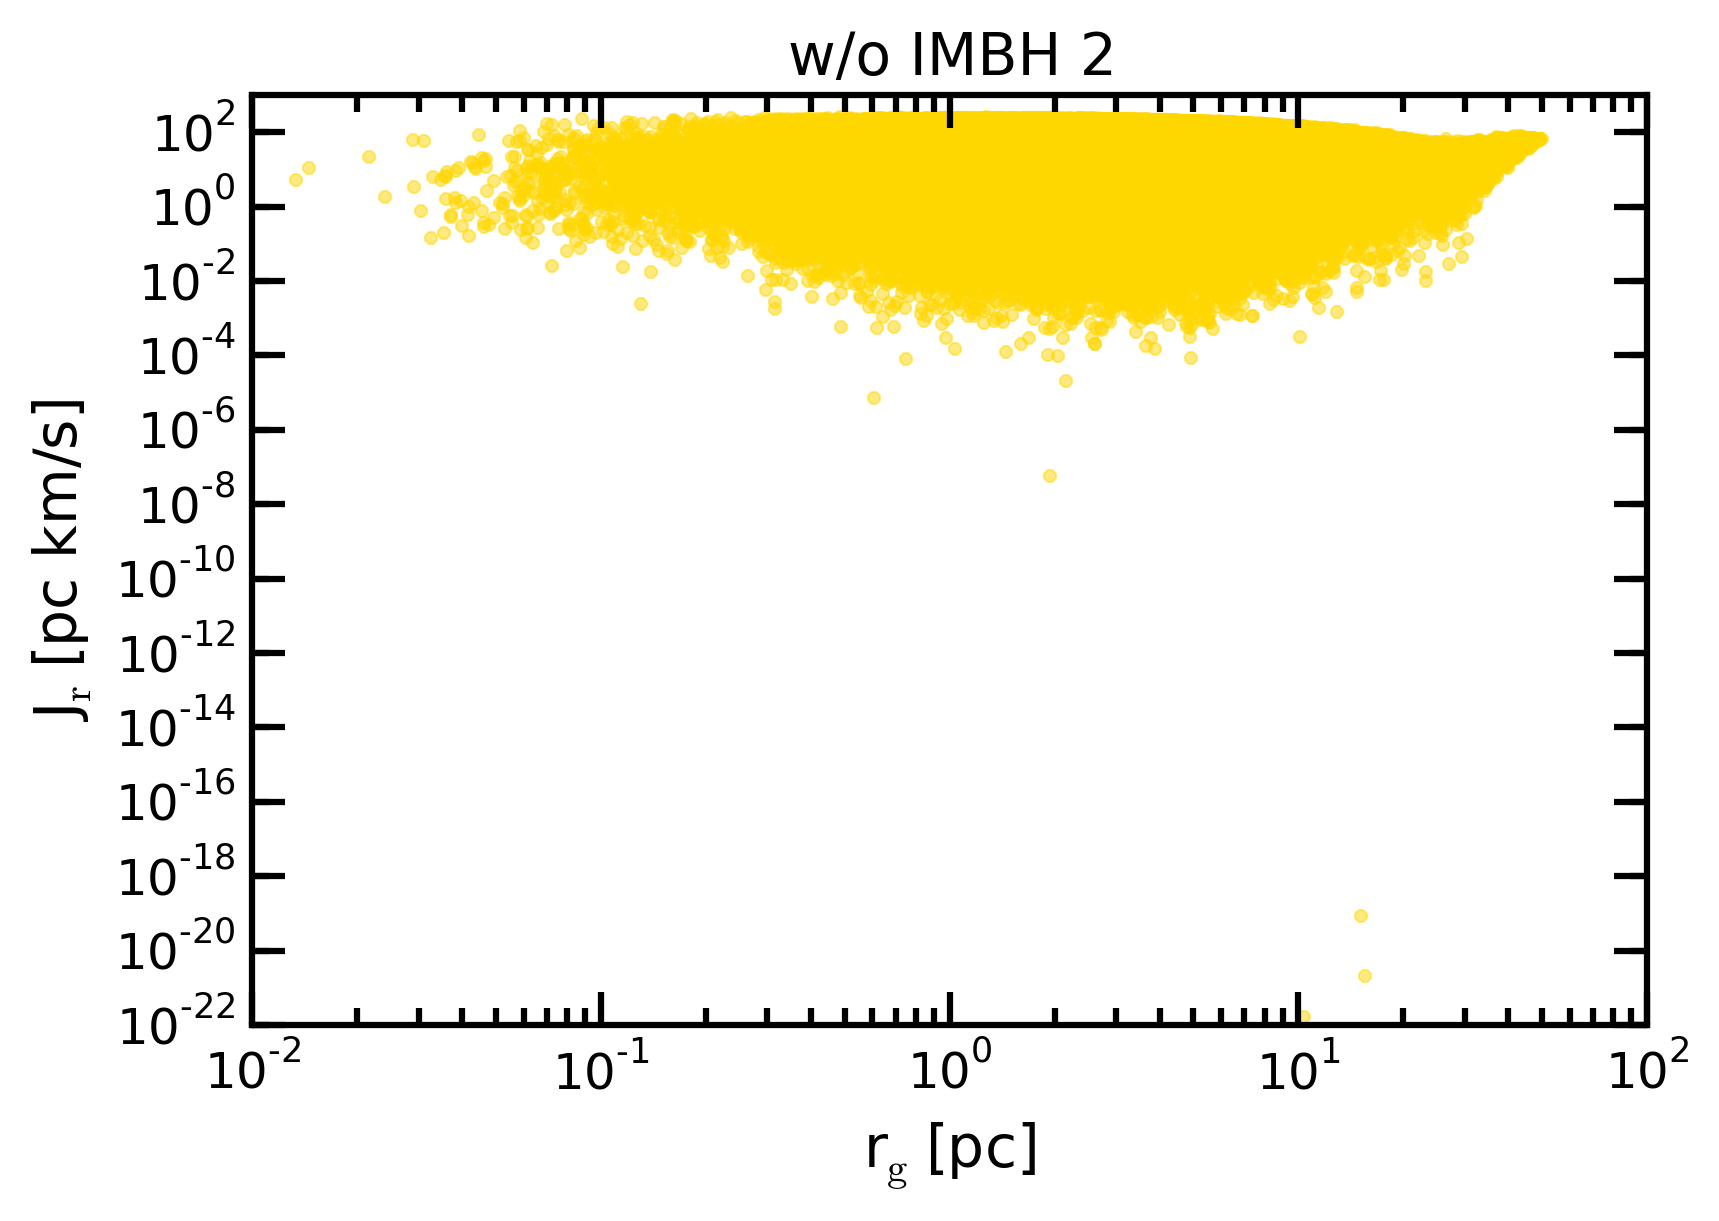
\includegraphics[width=\textwidth]{Plots/r_g_J_r_noIMBH2.png}
		\caption{SIM 4}
		\label{fig:r_g_J_r_noIMBH2}
	\end{subfigure}
	\caption{Radial action over guiding star radius with marked specific stars on loglog scale. All simulations have a similar shaped distributions except for the marked stars which are the specific ones. On the top right corner the shape of \ref{fig:E_J_r_hist_IMBH1} and \ref{fig:E_J_r_hist_IMBH2} is not gently rounded but there are single stars around it. On the lower left there are some extra stars which we identify as the stars with low radial action.}
	\label{fig:r_g_J_r}
\end{figure}
In graph \ref{fig:r_g_J_r} the radial actions are plotted over their guiding star distances. We highlight the stars of group 1 and group 2 taken from graph \ref{fig:E_J_r_hist} for SIM 1 and SIM 2. In general, there are several stars which have a really small guiding star radius (up to \(10^-5\) pc). In SIM 3 and SIM 4 only very few stars go below 0.1 pc. Another difference between the \acp{GC} with and the ones without \ac{IMBH} is that on the right border the lower end goes until very low radial actions for SIM 1 and SIM 2 (up to \(10^-6\) pc km/s) while SIM 3 and SIM 4 end there softly at about \(10^-2\) pc km/s. We investigate these different stars again in the radial action over energy plot to check their properties by colorcoding these different parts.

\begin{figure}
\centering
	\begin{subfigure}{0.475\textwidth}
	\centering
		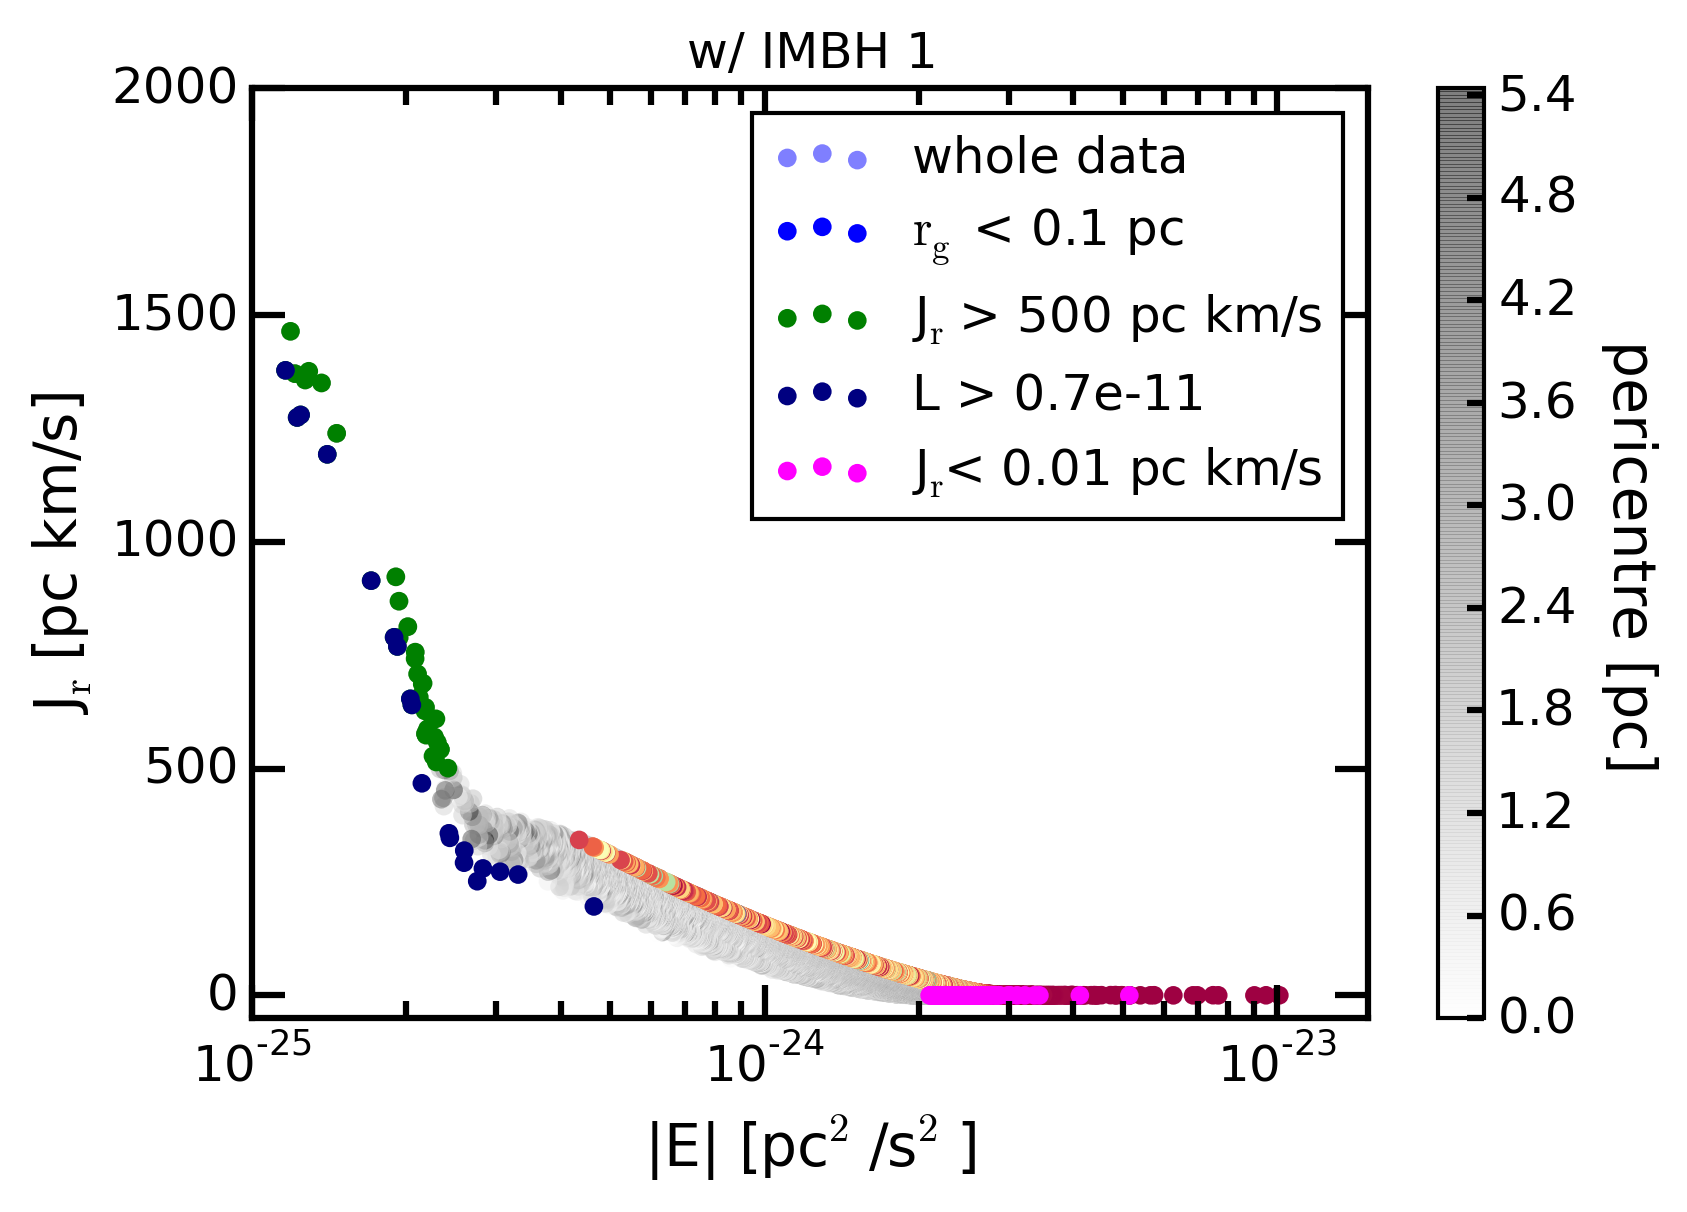
\includegraphics[width=\textwidth]{Plots/E_J_r_parts_IMBH1.png}
		\caption{SIM 1}
		\label{fig:E_J_r_parts_IMBH1}
	\end{subfigure}
	\hfill
	\begin{subfigure}{0.475\textwidth}
	\centering
		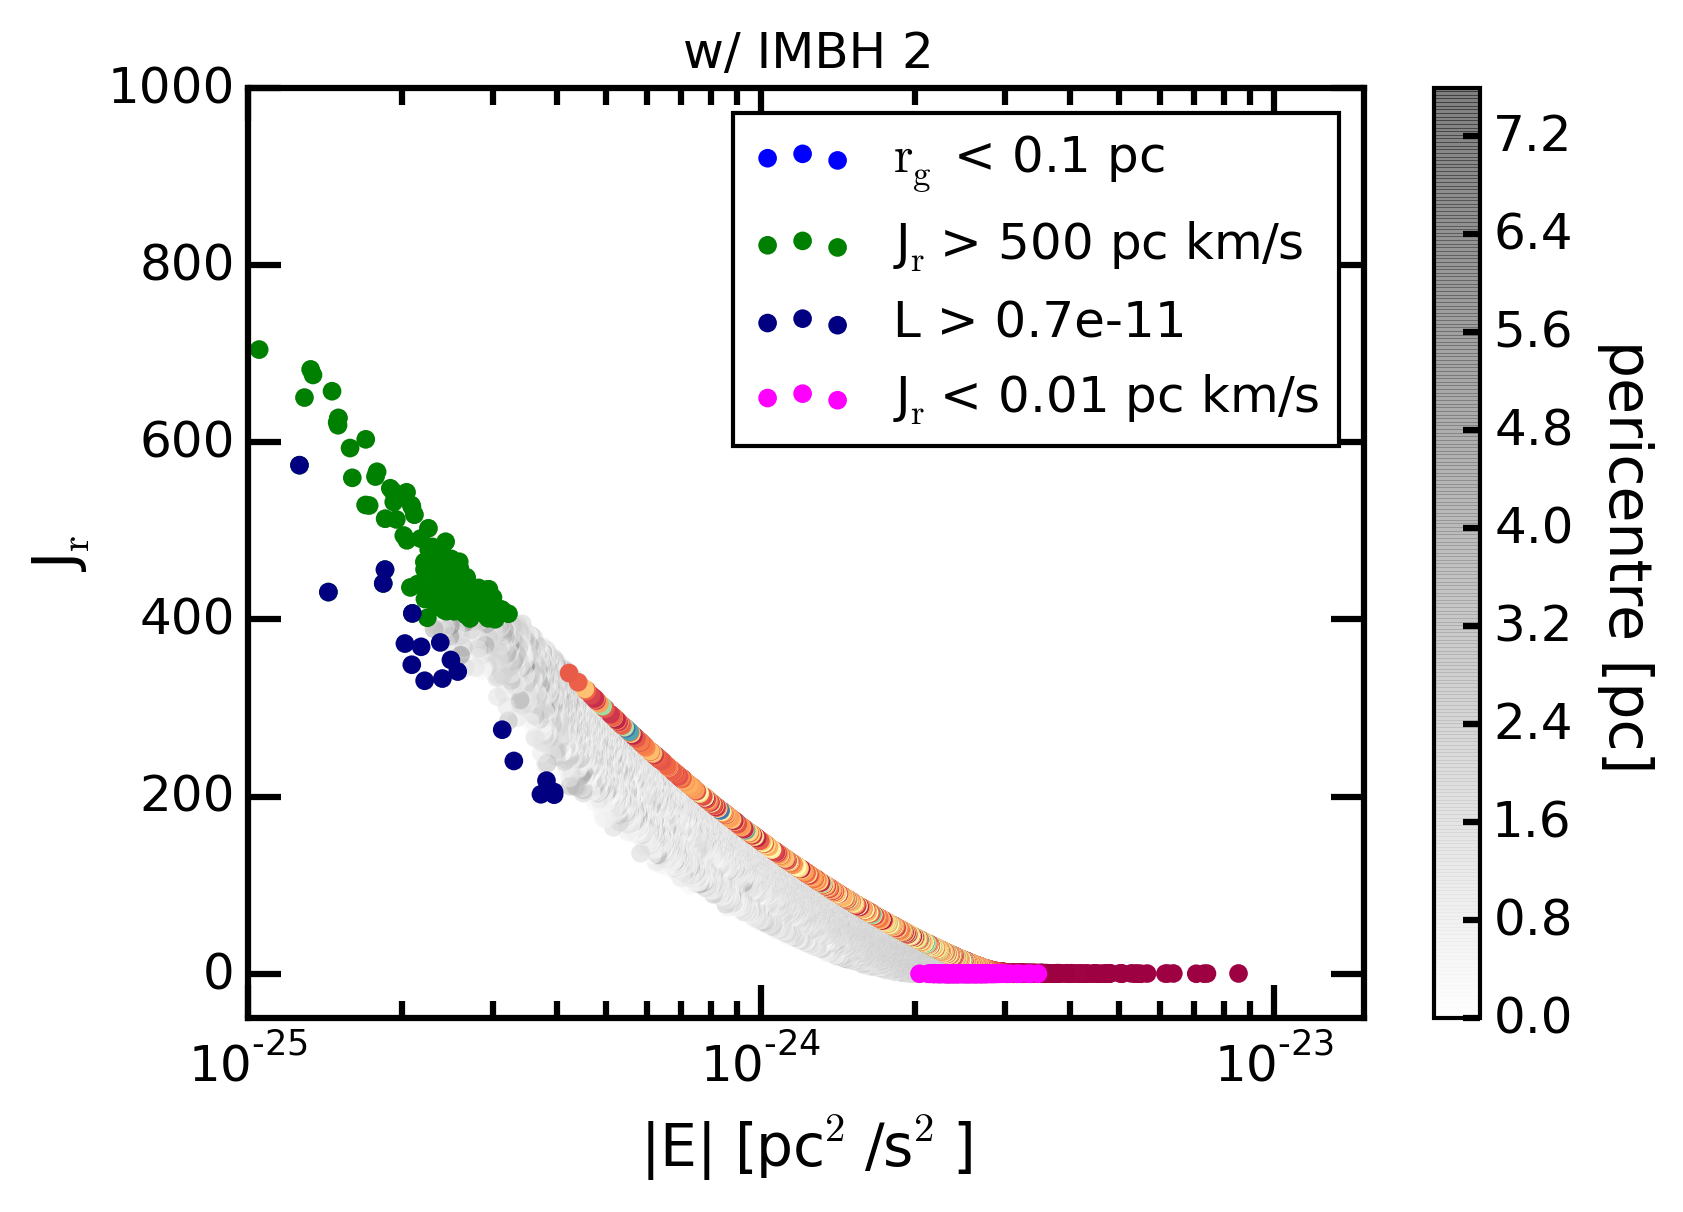
\includegraphics[width=\textwidth]{Plots/E_J_r_parts_IMBH2.png}
		\caption{SIM 2}
		\label{fig:E_J_r_parts_IMBH2}
	\end{subfigure}
	\vskip\baselineskip
	\begin{subfigure}{0.475\textwidth}
	\centering
		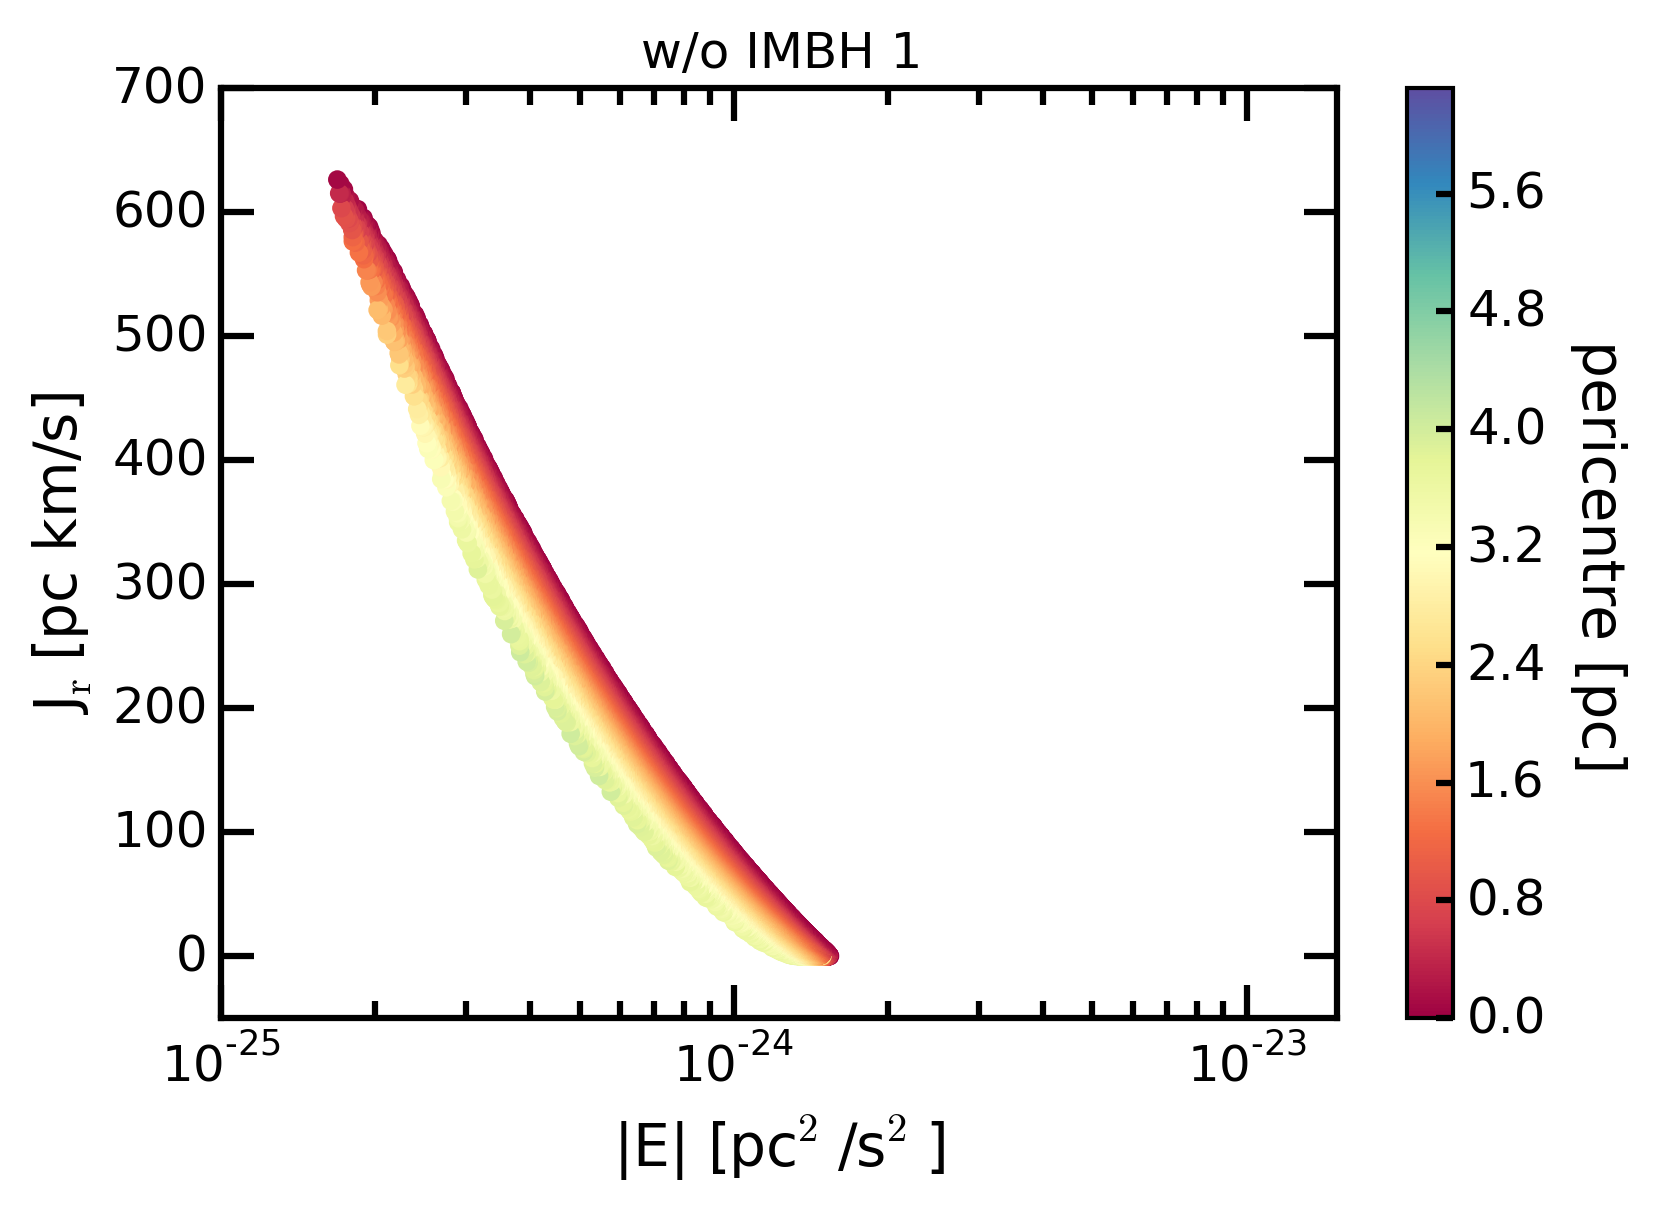
\includegraphics[width=\textwidth]{Plots/E_J_r_parts_noIMBH1.png}
		\caption{SIM 3}
		\label{fig:E_J_r_parts_noIMBH1}
	\end{subfigure}
	\hfill
	\begin{subfigure}{0.475\textwidth}
	\centering
		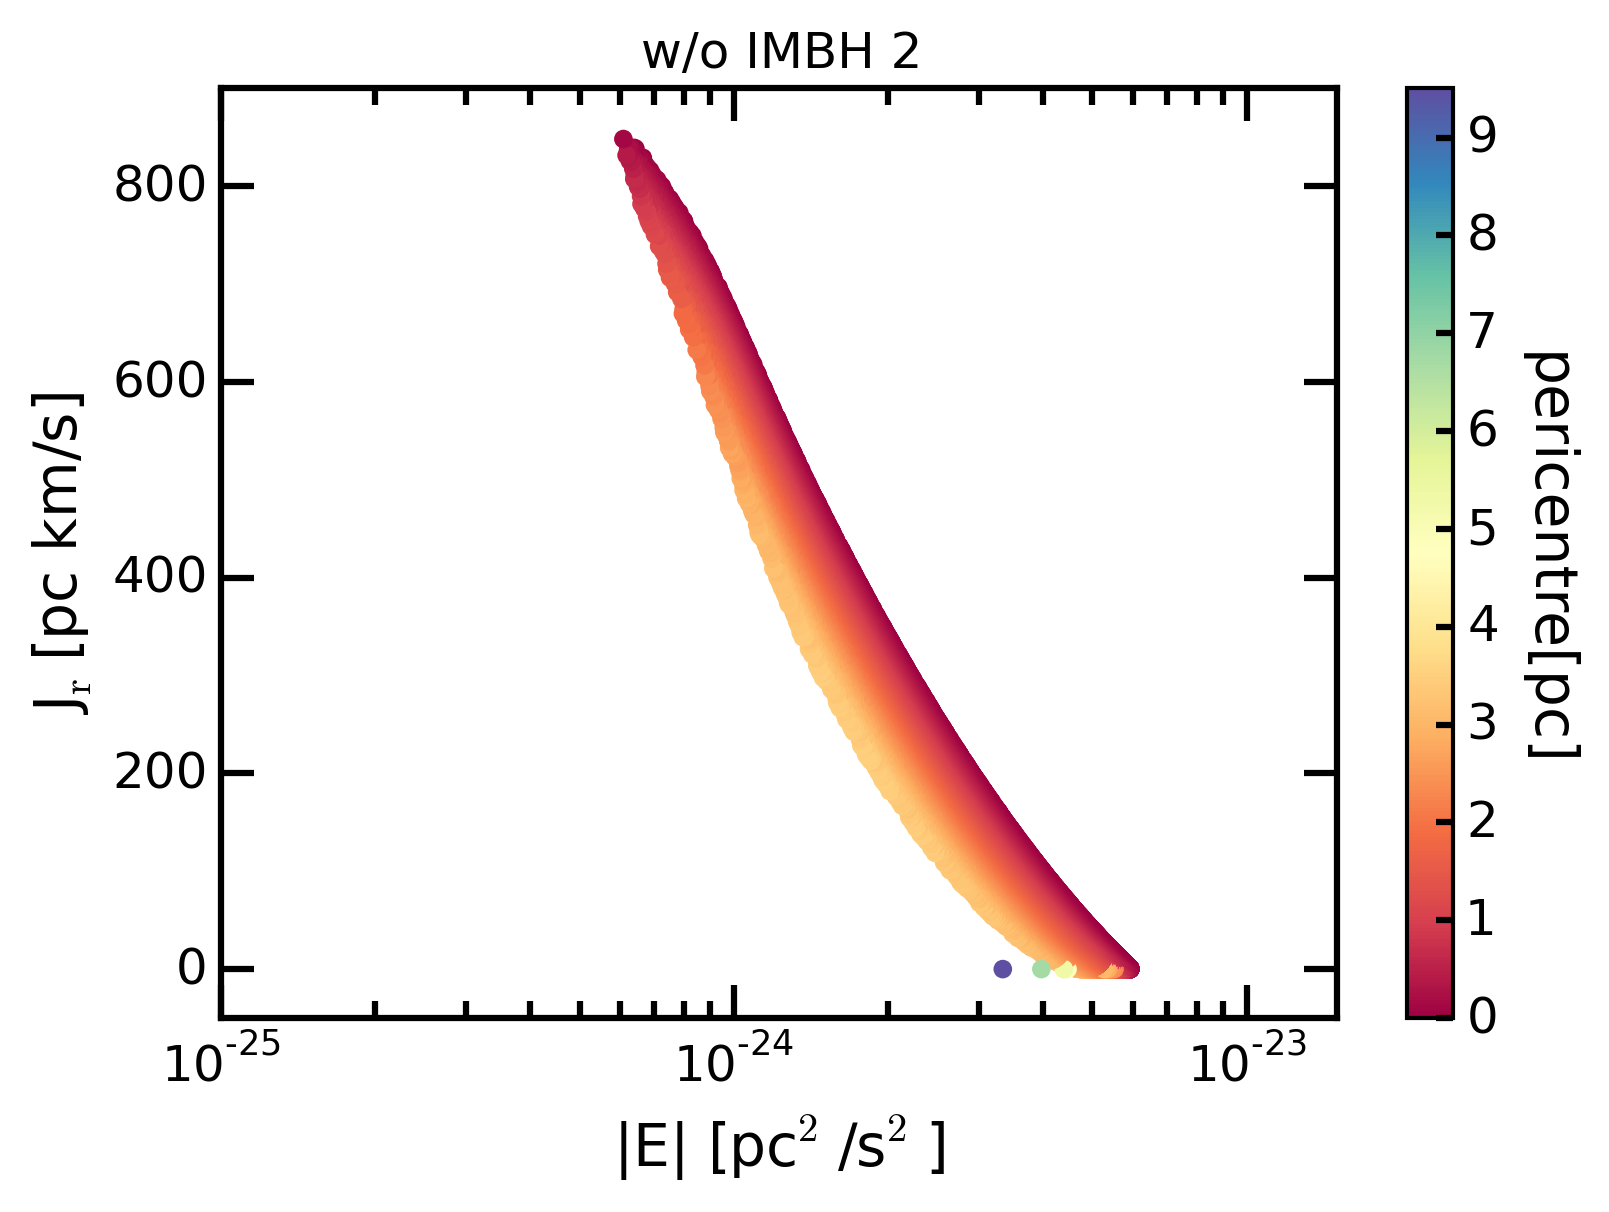
\includegraphics[width=\textwidth]{Plots/E_J_r_parts_noIMBH2.png}
		\caption{SIM 4}
		\label{fig:E_J_r_parts_noIMBH2}
	\end{subfigure}
\caption{Radial action over absolute energy plot color coded with different parts of the \acp{GC}.}
\label{fig:E_J_r_parts}
\end{figure}
In figure \ref{fig:E_J_r_parts} we can match the different parts of figure \ref{fig:r_g_J_r}. The grey part of figures \ref{fig:E_J_r_parts_IMBH1} and \ref{fig:E_J_r_parts_IMBH2} is the whole data color coded by the pericentre. The yellow to red part is the part where the guiding star radius is smaller than 0.1 pc again color coded by the pericentre. The green stars are the stars of group 2 while the pink stars contain stars of group 1. The blue stars are star with a high angular momentum (bigger than \(7\cdot 10^{-12}\) pc\(^2\)/s). If we subtract all color coded stars from this plot we get approximately the shape of SIM 3 and SIM 4. 
\subsection{Discussion \& future perspectives}
In summary we can say that we found clearly evidence of the \ac{IMBH} in the radial actions. To get there we made some simplified assumptions which should be investigated more precisely in an extended work. The density is the basis of our approach of the actions. Since we didn't find an analytical function we interpolated the binned densities and set the central density equal to the innermost density bin. Another attempt to get the density could be done by modelling Multi-Gaussian Expansion to the graph. But for this thesis we see the interpolation as sufficient since tests with some different densities do not destroy the figures of section \ref{results}. \par Additional inaccuracy of the results rises due to different simulations for \acp{GC} with and without \ac{IMBH}. Since they have different initial conditions and conditions throughout the simulating process we can not compare them directly. Especially the radial actions can not be compared since they are mass dependent. We see the differences directly in the scatter plots (figures \ref{fig:position_scatter} and \ref{fig:velocity_scatter}) and in the anisotropy due to different truncation prescriptions. In further investigations we should consider using simulations with same conditions despite only the absence of an \ac{IMBH} in one of the simulations. \par Some physical assumptions have been that actions stay totally constant over time or rather that we have only looked at them at the time of the snapshot (despite a few stars for which we integrated the orbit and have looked at the time evolution of their integrals of orbits). Changing actions 

alles was geplottet ist ist spezifisch (ohne masse)
half moon not directly spatially connected to imbh (plot mit color coding pericentre einfügen) probably only specific to the simulation
do the same distinguishing the mass of the stars\\
redo the work with only observational-like data